% \documentclass[aspectratio=169,notes]{beamer}
\documentclass[aspectratio=169]{beamer}
\usetheme[faculty=phil]{fibeamer}
\usepackage{polyglossia}
\setmainlanguage{english} %% main locale instead of `english`, you
%% can typeset the presentation in either Czech or Slovak,
%% respectively.
\setotherlanguages{russian} %% The additional keys allow
%%
%%   \begin{otherlanguage}{czech}   ... \end{otherlanguage}
%%   \begin{otherlanguage}{slovak}  ... \end{otherlanguage}
%%
%% These macros specify information about the presentation
\title[MaM]{Mechanics and Machines, CAD Assembly 1} %% that will be typeset on the
\subtitle{Bottom-Up approach
\\ Basics \\ \ 
         } %% title page.
\author{Oleg Bulichev}
%% These additional packages are used within the document:
\usepackage{ragged2e}  % `\justifying` text
\usepackage{booktabs}  % Tables
\usepackage{tabularx}
\usepackage{tikz}      % Diagrams
\usetikzlibrary{calc, shapes, backgrounds}
\usepackage{amsmath, amssymb}
\usepackage{url}       % `\url`s
\usepackage{listings}  % Code listings
% \usepackage{subfigure}
\usepackage{floatrow}
\usepackage{subcaption}
\usepackage{mathtools}
\usepackage{todonotes}
\usepackage{fontspec}
\usepackage{multicol}
\usepackage{pdfpages}
\usepackage{wrapfig}
\usepackage{animate}
\usepackage{booktabs}
\usepackage{multirow}
% \usepackage{graphicx}
\usepackage{colortbl}

\graphicspath{{resources/}}
\frenchspacing

\setbeamertemplate{caption}[numbered]
\usetikzlibrary{graphs}

% \usepackage[backend=biber,style=ieee,autocite=footnote]{biblatex}
% \addbibresource{biblio.bib}
% \DefineBibliographyStrings{english}{%
%   bibliography = {References},}

\newcommand{\oleg}[2][] {\todo[color=red, #1] {OLEG:\\ #2}}
\newcommand{\fbckg}[1]{\usebackgroundtemplate{\includegraphics[width=\paperwidth]{#1}}}%frame background

\usepackage[framemethod=TikZ]{mdframed}
\newcommand{\dbox}[1]{
\begin{mdframed}[roundcorner=3pt, backgroundcolor=yellow, linewidth=0]
\vspace{1mm}
{#1}
\vspace{1mm}
\end{mdframed}
}

\begin{document}
\setlength{\abovedisplayskip}{0pt}
\setlength{\belowdisplayskip}{0pt}
\setlength{\abovedisplayshortskip}{0pt}
\setlength{\belowdisplayshortskip}{0pt}

\fbckg{fibeamer/figs/title_page.png}
\frame[c]{\setcounter{framenumber}{0}
    \usebeamerfont{title}%
    \usebeamercolor[fg]{title}%
    \begin{minipage}[b][6.5\baselineskip][b]{\textwidth}%
        \textcolor{black}{\raggedright\inserttitle}
    \end{minipage}
    % \vskip-1.5\baselineskip

    \usebeamerfont{subtitle}%
    \usebeamercolor[fg]{framesubtitle}%
    \begin{minipage}[b][3\baselineskip][b]{\textwidth}
        \raggedright%
        \insertsubtitle%
    \end{minipage}
    \vskip.25\baselineskip
}
%   \frame[c]{\maketitle}

\fbckg{fibeamer/figs/common.png}

\note{\scriptsize \begin{itemize}
        \item \
    \end{itemize}}

\note{
   \ 
}

\begin{frame}[c]{Assemblies}
\framesubtitle{}
    \centering
    \Huge
    Introductory words
\end{frame}

\begin{frame}[t]{Basics (1)}
    \framesubtitle{Video + \href{https://disk.yandex.ru/d/7ZBj1dYl2SWxjA}{parts}}
    \vspace{-0.6cm}
    \begin{figure}[H]
        \href{https://disk.yandex.ru/i/eTpcseXL44F6jQ}{
            \centering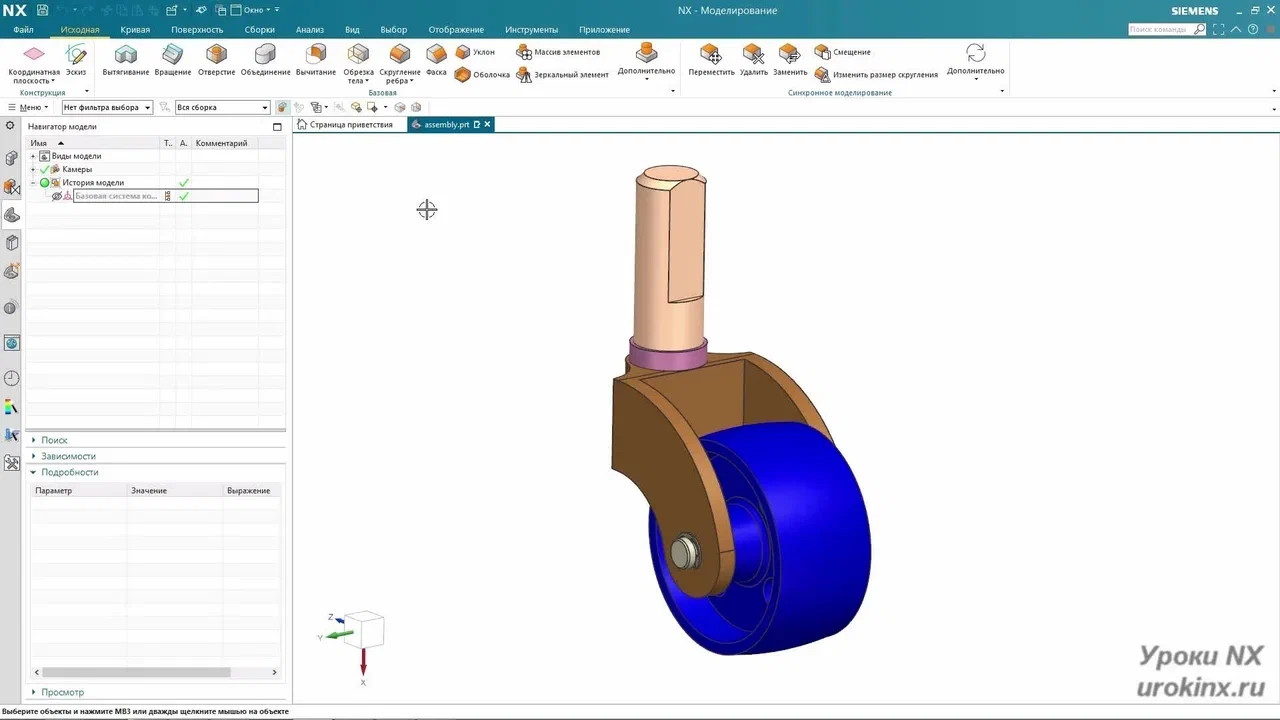
\includegraphics[height=6cm,width=1\textwidth,keepaspectratio]{1.png}}
        % \caption{Click on a picture for a video}
        \label{fig:1}
    \end{figure}
\end{frame}

\begin{frame}[t]{Task 1}
\framesubtitle{}
    \begin{figure}[H]
        \centering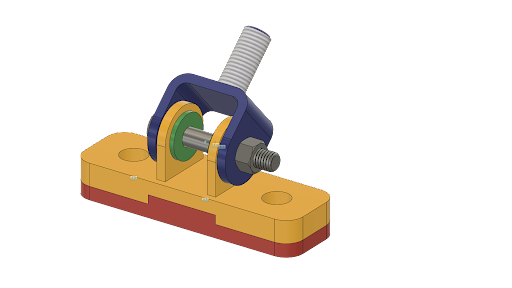
\includegraphics[height=5cm,width=1\textwidth,keepaspectratio]{task1.png}
        \caption*{Make an assembly as in figure. \href{https://disk.yandex.ru/d/7ZBj1dYl2SWxjA}{Parts here}}
        \label{fig:task1.png}
    \end{figure}
\end{frame}

\begin{frame}[t]{Task 2}
    \framesubtitle{}
        Import step file and make a moveable assembly. \href{https://disk.yandex.ru/d/7itUHTJBdrYhzg}{Parts here}
    \end{frame}

    \begin{frame}[t]{Basics (2)}
        \framesubtitle{Video + \href{https://disk.yandex.ru/d/7ZBj1dYl2SWxjA}{parts}}
        \vspace{-0.6cm}
        \begin{figure}[H]
            \href{https://disk.yandex.ru/i/kbz5Hqkpsvte8w}{
                \centering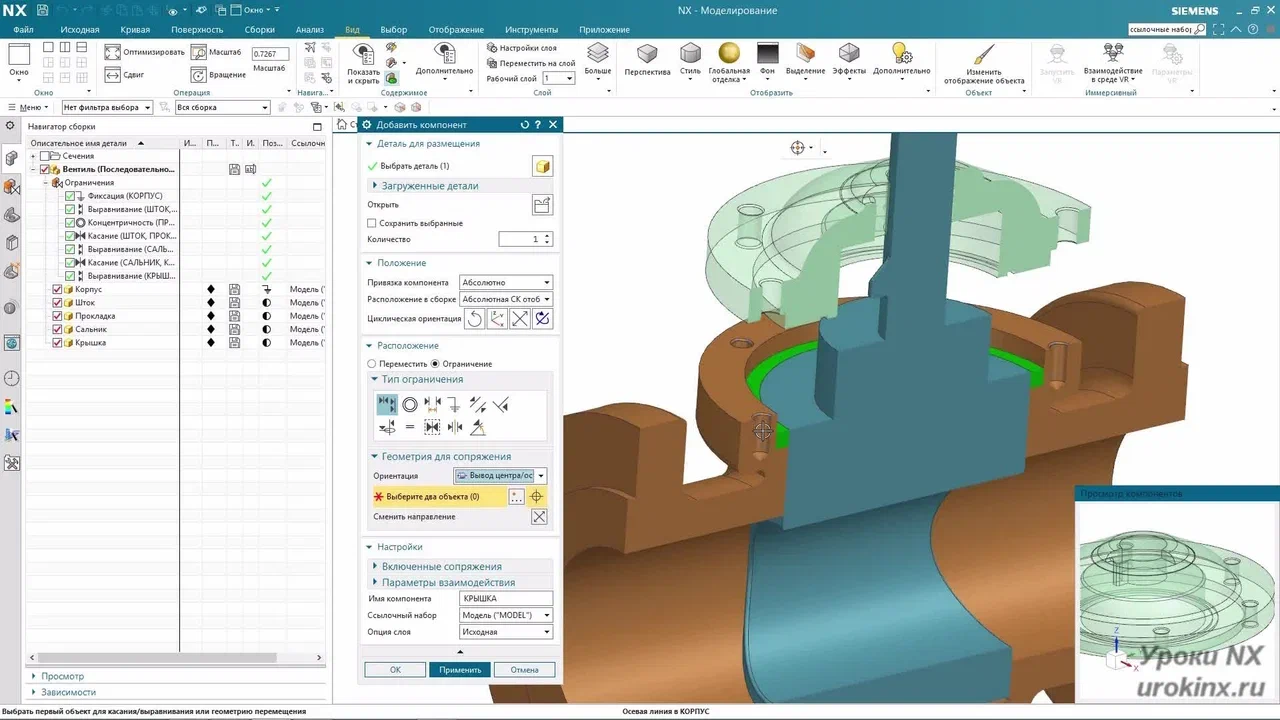
\includegraphics[height=6cm,width=1\textwidth,keepaspectratio]{2.png}}
            % \caption{Click on a picture for a video}
            \label{fig:2}
        \end{figure}
    \end{frame}

\fbckg{fibeamer/figs/last_page.png}
\frame[plain]{}

\end{document}